\documentclass[11pt,a4paper]{article}
\usepackage[utf8]{inputenc}
\usepackage{a4wide}
\usepackage{amsmath}
\usepackage{amsfonts}
\usepackage{amssymb}
\usepackage{graphicx}

\newcommand{\mydiv}{\ensuremath{\operatorname{div}}}
\newcommand{\myvec}[1]{\ensuremath{\mathbf{#1}}}
\newcommand{\gvec}[1]{\ensuremath{\overset{\rightarrow}{#1}}}
\newcommand{\scal}[2]{\ensuremath{\langle #1 , #2 \rangle}}

\title{Distance, curvature }
\author{Hugues Talbot}

\begin{document}
\maketitle
	
	
	\section{Normals and curvature}
	
	There is a deep link between the evolution of the normal vector along a curve and its curvature .
	
	Let $C$ be a planar curve. To define the curvature at a point, we can consider
	the case of a straight line. We can admit that in this case the curvature is zero along the line. For a portion of a circle, the curvature is defined to be inversely proportional to the radius of the circle:
	
	\begin{equation}
	\kappa = \frac{1}{R}
	\end{equation}
	
		\begin{figure}
			\centering
			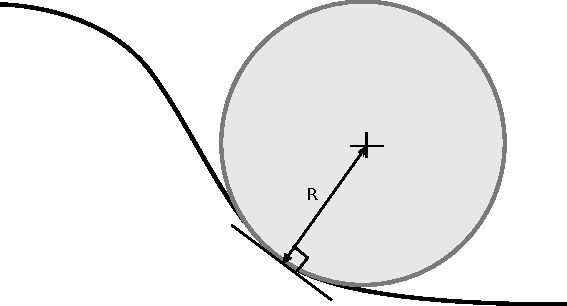
\includegraphics[width=0.5\textwidth]{Drawings/Osculating.pdf}
			\caption{The notion of an osculating circle (best local approximation) defines the curvature as the inverse of the radius of the circle.\label{fig:oscul}}
		\end{figure}
	
	More precisely, for any curve, we can locally approximate a sufficiently regular curve (${\cal C}^2$ is enough) at a point by a circle that best approximates it locally (see Fig.~\ref{fig:oscul}. This circle is tangent to $C$ and is called an {\em osculating circle}. The radius of this circle defines the curvature.
	

	
	Another way to define the curvature is to consider a point moving at a constant speed along the curve $C$. The variation of the tangent vector along the curve defines the curvature. This is equivalent to specifying the acceleration of the point.
	
	
	\begin{equation}
	\kappa = \frac{d \mathbf{T}}{ds},
	\end{equation}
	
	where $s$ is a parametrisation of the curve. Both definition of the curvature
	are in fact equivalent (see Fig.~\ref{fig:theta}). 
	
	\begin{figure}
		\centering
		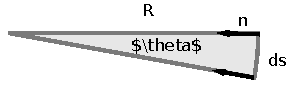
\includegraphics[width=0.3\textwidth]{Drawings/theta.pdf}
		\caption{We can write $\sin d\theta \approx d\theta = \frac{ds}{R}$. As ds tends to zero, we have $R = \frac{d\theta}{ds} = \frac{d \mathbf{T}}{ds}$.\label{fig:theta}}
	\end{figure}
	
	
	\section*{Parametrisation}
	
	Let $\gamma(t)$ be a parametrisation of the curve $C$, i.e.
	
	\begin{equation}
	\gamma(t) = (x(t),y(t))
	\end{equation}
	
	This defines the position of a point on the curve over time. We assume an injective parametrisation, i.e. such that
	the speed $\gamma'(t)$ is never zero. This means 
	
	\begin{equation}
	\forall t, \|\gamma'(t)\|^2 = x'(t)^2 + y'(t)^2 > 0 
	\end{equation}
	
	In this case, we can re-paramametrise the curve with curvilinear abcissa $s$ in such a way that the speed is constant and equal to one.
	
	\begin{equation}
	\forall s, \gamma'(s)^2 = x'(s)^2 + y'(s)^2 = 1
	\end{equation} 
	
	In this parametrisation, $\gamma'$ is the unit tangent velocity vector $\mathbf{T}$. If $\mathbf{N}$ is the unit normal vector to the curve, we have
	
	\begin{equation}
	\mathbf{T}'(s) = \kappa(s)\mathbf{N}(s)
	\end{equation}
	
	We note that instead of deriving the unit tangent vector, we can also consider deriving the unit normal vector. This is because $\mathbf{N}$ is $\mathbf{T}$ rotated by $\frac{\pi}{2}$, i.e. $\mathbf{N}(x,y) = (-y'(s),x'(s))$. This yields
	
	\begin{equation}
	\mathbf{N}'(s) = \kappa(s)\mathbf{T}(s)
	\end{equation}
	
	We will make use of that fact in the next section.
	
	\section*{Level sets}
	
	In imaging it can be difficult to represent a parametric curve because of discretization effects. It is common to
	represent it by a {\em level set} (see Fig.~\ref{fig:level_set}).
	
	\begin{figure}
		\centering
		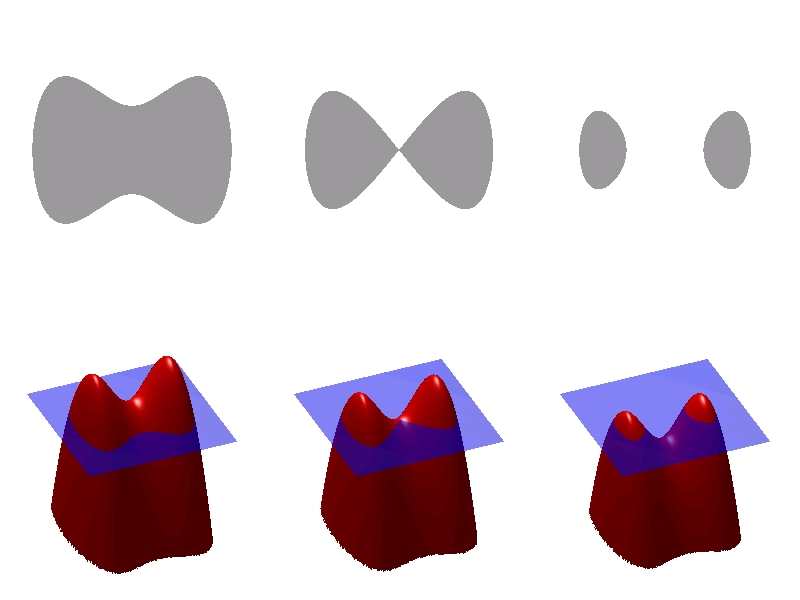
\includegraphics[width=0.5\textwidth]{Images/Level_set_method.jpg}
		\caption{Representing a curve by a level set.\label{fig:level_set}}
	\end{figure}
	
	Let $\phi(x,y)$ be a ${\cal C}^2$ function in a domain $\Omega$. We define the curve $\Gamma$ as the zero-level-set of this function
	
	\begin{equation}
	\Gamma = \{(x,y), \phi(x,y) = 0\}
	\end{equation}
	
	$\Gamma$ is a set and no longer a parametrized curve, however we can manipulate it by working on the underlying $\phi$ function. This is the main idea behind the level-set method~\cite{Sethian-level-sets-1999}.
	

	
	\section*{Level sets and curvature}
	
	Curvature is easy to define in the level set case. For any point $(x,y)$ in $\Omega$, $\nabla \phi (x,y)$ is the gradient at $(x,y)$. If we consider the level-set at $(x,y,\phi(x,y))$, i.e. the curve that passes through $(x,y)$ at level $\phi(x,y)$, 
	then $\nabla \phi(x,y)$ is the normal vector to this curve at $(x,y)$. The unit normal is given by
	
	\begin{equation}
	\mathbf{n}(x,y) = \frac{\nabla \phi}{|\nabla \phi|}(x,y)
	\end{equation}
	
	The curvature is given by the derivative of this expression. However this is a multidimensional derivative. Since $\nabla \phi$ is a vector, we must use the divergence operator $\nabla . \mathbf{F} \equiv \sum_i^d \frac{\partial \mathbf{F}}{\partial x_i}$:
	
	\begin{equation}
	\kappa = \nabla . \frac{\nabla \phi}{|\nabla \phi|}
	\end{equation}
	
	This is in particular true for the computation of the curvature of $\Gamma$. 
	
		\begin{figure}
			\centering
			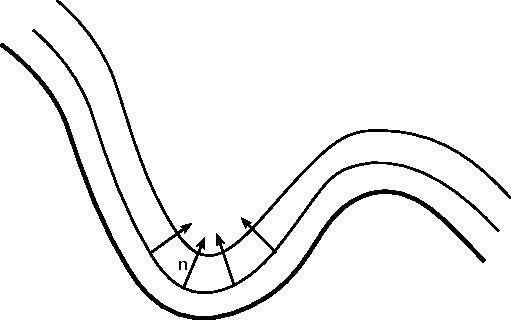
\includegraphics[width=0.5\textwidth]{Drawings/Distance.pdf}
			\caption{The faster the normal evolves along a curve, the higher the curvature.}
		\end{figure}
		
	\section{Application to our problem}
	
Here we assume a non-convex territory with two nested surfaces as borders. Every point $p$ of the territory is associated with a value $\omega(p)$ so that $\omega(p) = 0$ if $p$ belongs to the inner surface, and $\omega(p) = 1$ on the outer surface. Numerically, $\omega$ can for example be computed from solving the electrostatic Poisson equation, i.e. a random walker. Our formulations and illustrations are in 2D but carry over to 3D without significant changes.


Let $[p_1p_2]$ be the segment defined by the points $\{p_1, p_2\}$. We want to define how to sample this segment, so that we can conclude with high confidence whether or not the whole segment is located inside a non-convex territory. The number of samples ($n + 1$), shall be optimized in order to avoid too many tests (minimize computation time) but also to guarantee the result within a reasonable tolerance (maximize test accuracy).

	\subsection{First approach} \label{firstaproach}

We can estimate $n$, the number of samples along the segment, from:
\begin{equation}
n \propto \frac{|p_2 - p_1|}{R}
\end{equation}
$R$ is an approximation of the local radius of curvature along the segment by estimating the divergence at each point $p_1$ and $p_2$, called $\kappa_1$ and $\kappa_2$ respectively :
\begin{equation}
R = \max(|\frac{1}{\kappa_1}|, \frac{1}{|\kappa_2|})
\end{equation} 
The figure \ref{example} illustrates the relationship between $D = |p_2 - p_1|$, $R_1= \frac{1}{|\kappa_1|}$, $R_2=\frac{1}{|\kappa_2|}$ and $n$. 
\begin{figure}[h!]
\centering
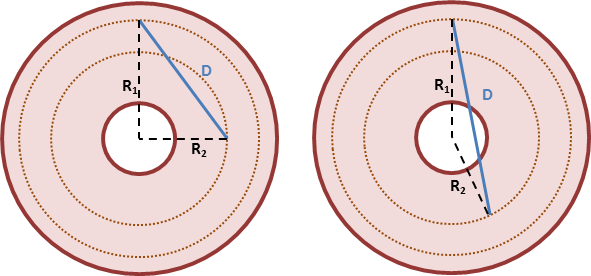
\includegraphics[width=0.5\textwidth]{Drawings/CurvatureTestExample.png}
\caption{When $D$ becomes larger relatively to $\max(|R_1, R_2|)$, the value of $n$ is also higher to detect if the segment crosses the perfusion territory.}
\label{example}
\end{figure}

The divergence of a a continuously differentiable vector field $\myvec{w}=(w_x,w_y)$ is equal to the scalar value function:
\begin{equation}
\mydiv (\myvec{w}) = (\frac{\partial}{\partial x}, \frac{\partial}{\partial y}) \cdot (w_x, w_y) 
\end{equation}
\begin{equation}
\mydiv (\myvec{w}) = \left( w_x(x, y) - w_x(x-1, y) \right) + \left( w_y(x, y) - w_y(x, y - 1) \right).
\end{equation}

Since we are interested in estimating a curvature, the field $\myvec{w}$ is the normalized gradient of $\omega$.
\begin{equation}
w_x = \frac{\nabla_x \omega}{\|\nabla \omega\|} = \frac{\omega (x + 1, y) - \omega (x, y)}{\sqrt{(\nabla_x\omega)^2 + (\nabla_y\omega)^2}}
\end{equation}
and
\begin{equation}
w_y = \frac{\nabla_y \omega}{\|\nabla \omega\|} = \frac{\omega (x, y + 1) - \omega (x, y)}{\sqrt{(\nabla_x\omega)^2 + (\nabla_y\omega)^2}}
\end{equation}	

This approach does not take into account the position of $p_1$ and $p_2$ within the territory, and so it is easy to find counter-examples where this approach fails.

\subsection{Second approach}

%We are in the case of measuring the curvature along a segment, so we could use the segment information within an iterative %process.
Here we consider an iterative process to take into account the curvature along a segment.

\subsubsection{Interpolating the point along the segment line that crosses the concavity} \label{subsec}
We calculate the distances $\lambda_1,\lambda_2$ that solves:
\begin{equation}
\omega (p_1) + \lambda_1 \scal{\nabla\omega(p_1)}{\overset{\rightarrow}{p_1p_2}} =  0,
\end{equation}
and symmetrically for $\lambda_2$.


Then we select:
\begin{equation}
\lambda = \min(\lambda_1, \lambda_2)
\end{equation}
to obtain :
\begin{equation}
n = \Bigl\lceil \frac{1}{\lambda} \Bigr\rceil,
\end{equation}
where $\lceil.\rceil$ denotes the ceiling operator, i.e. the function that maps a real number to the smallest integer that is larger or equal to it.

If  $\lambda < 0$ or $\lambda > 1$, it means the line $(p_1p_2)$ crosses the concavity outside of the segment $[p_1p_2]$. We could consider that there is actually no need of refining the test along the segment. But we have to keep in mind that this interpretation comes only from a linear local approximation. In Fig.~\ref{fig:cec}, we show a counter-example, where this approach fails.

\begin{figure}[h!]
			\label{spe issue}
			\centering
			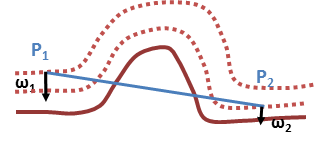
\includegraphics[width=0.25\textwidth]{Drawings/CurvatureTestExample1.png}
			\caption{Specific situation where the local gradient doesn't help detecting the concavity.\label{fig:cec}}
\end{figure}
Also, this method would fail for any case where the dot product $\scal{\nabla \omega(p_1)}{\overset{\rightarrow}{p_1p_2}} \simeq 0$, and in some specific situations such as the figure \ref{spe issue}. Hence we need to define a global boundary:
\begin{equation}
n \geq \frac{||\overset{\rightarrow}{p_1p_2}||}{R_{\text{max}}}
\end{equation}
with $R_{\text{max}}$ the maximal curvature radius of both inner and outer surfaces.

Note: if the segmentation is noisy, we might actually measure non-physical very high curvatures, i.e. $R_{max}$ close to zero, hence it is necessary to consider a tolerance $s$ so that 
\begin{equation}
R_{max}^* = R_{max} - s
\end{equation}

\begin{figure}[h!]
			\centering
			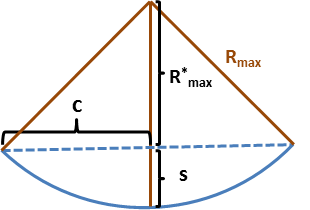
\includegraphics[width=0.25\textwidth]{Drawings/CurvatureTolerance.png}
			\caption{The maximally inscribed radius and tolerance s define a semi-cord $c$.}
\end{figure}

The semi-cord $c$ defined by $R_{max}^*$ and $s$ is calculated as:
\begin{equation}
c = \sqrt{R_{max}^2 - R_{max}^{*2}}
\end{equation} 
That can be simplified as:
\begin{equation}
c = \sqrt{R_{max}^2 - (R_{max} - s)^2}
\end{equation}
The global boundary follows this tolerance:
\begin{equation}
n \geq \frac{||\overset{\rightarrow}{p_1p_2}||}{c}
\end{equation}

We take the largest $n$ between maximal curvature and gradient method. This provides a robust sampling definition considering both local and global informations, see figure \ref{test sampling}.
\begin{figure}[h!]
			\label{test sampling}
			\centering
			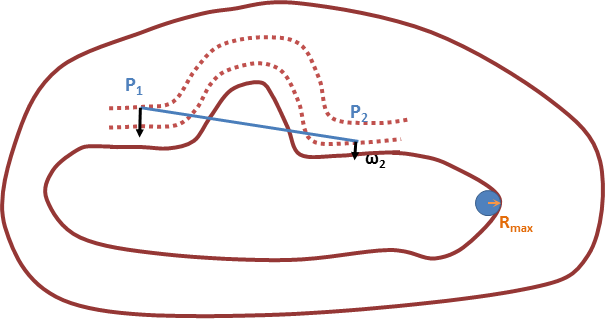
\includegraphics[width=0.35\textwidth]{Drawings/CurvatureTestExample2.png}
			\caption{In this situation, considering the global maximum curvature will allow us to detect the concavity between $p_1$ and $p_2$.}
\end{figure}

\subsubsection{Estimating a sampling distance from the projection of the border}


\begin{figure}
	\centering
	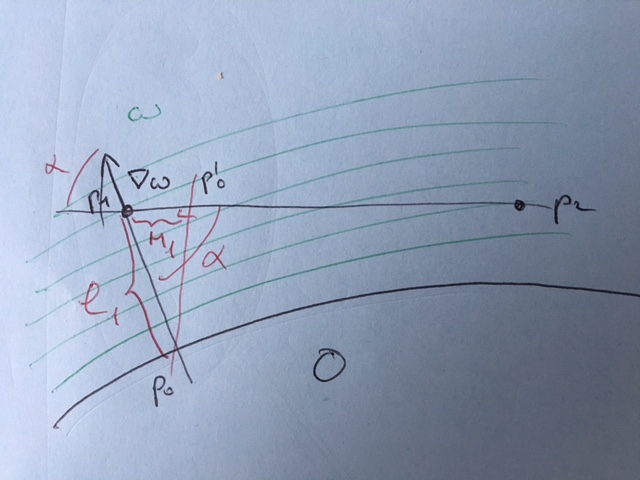
\includegraphics[width=0.7\textwidth]{Images/blue_doodle.jpg}
	\caption{We want to measure length $M_1$ as a way to sample the segment $[p_1p_2]$.\label{fig:findM}}
\end{figure}


Given $p_1$ and $p_2$, we want to find length $M_1$ in Fig.~\ref{fig:findM} from local information.

First we denote $p_0$ the intersection of the steepest descent from $p_1$ with the 0-surface, the surface where $\omega=0$.  since $\nabla \omega(p_1)$ and $\gvec{p_0p_1}$ are co-linear, to first order we can write

\begin{equation}
\nabla \omega(p_1) \approx \frac{\omega(p_0) - \omega(p_1)}{\gvec{p_1p_0}}
\end{equation}



Point $p_0$ is actually unknown, but $\omega(p_0) = 0$, so we have:
\begin{equation}
\gvec{p_1p_0} \approx \frac{- \omega(p_1)}{\nabla\omega(p_1)}
\end{equation}
Then we can project this vector $\gvec{p_1p_0}$ on the segment $gvec{p_1p_2}$:
\begin{equation}
M_1 = \frac{\scal{\gvec{p_1p_0}}{\gvec{p_1p_2}}}{||\gvec{p_1p_2}||}
\end{equation}



%Hugues's proposition
%\begin{equation}
%\scal{\nabla \omega(p_1)}{\gvec{p_0p_1}} = \|\nabla \omega(p_1)\| \|\gvec{p_0p_1}\|  \approx \omega(p_1) - \omega(p_0),
%\end{equation}
%Point $p_0$ is actually unknown, but $\omega(p_0) = 0$, so with $l_1=\|\gvec{p_0p_1}\|$, we have:
%
%\begin{equation}
%l_1 = \frac{\omega(p_1)}{\|\nabla \omega(p_1)\|}
%\end{equation}



Note: the research of $\gvec{p_1p_0}$ is the Newton method for finding a root, so this estimate can be iteratively refined if need be, although in this case it is not probably very useful. 
%We now want to project $l_1$ onto the line $(p_1p_2)$ to find the distance $M_1$. We note
%
%\begin{align}
%M_1 & = \|\gvec{p_0p_1}\|\cos \alpha = l_1 \cos \alpha\\
%\scal{\nabla \omega(p_1)}{\gvec{p_2p_1}} & = \|\nabla \omega(p_1)\|\|\gvec{p_2p_1}\|\cos \alpha
%\end{align}
%
%finally:
%
%\begin{equation}
%M_1 = l_1 \frac{\scal{\nabla \omega(p_1)}{\gvec{p_2p_1}}}{\|\nabla \omega(p_1)\|\|\gvec{p_2p_1}\|}.
%\end{equation}

Symmetrically we can find $M_2$, by first denoting $p_0$ the intersection of the steepest descent from $p_2$ with the 0-surface, and minding the vector reversal: 

%\begin{equation}
%l_2 = \frac{\omega(p_2)}{\|\nabla \omega(p_2)\|}
%\end{equation}
%
%\begin{equation}
%M_2 = l_2 \frac{\scal{\nabla \omega(p_2)}{\gvec{p_1p_2}}}{\|\nabla \omega(p_2)\|\|\gvec{p_1p_2}\|}.
%\end{equation}
\begin{equation}
M_2 =  \frac{\scal{\gvec{p_2p_0}}{\gvec{p_2p_1}}}{||\gvec{p_2p_1}||}.
\end{equation}

From this we take the smallest projection:
\begin{equation}
d_{\text{proj}} = \min(M_1,M_2)
\end{equation}

This distance $d_{\text{proj}}$ is a geometrically meaningful way to sample the segment, so $n$ can be defined as:
\begin{equation}
n = \Bigl\lceil\frac{||\gvec{p_1p_2}||}{d_{\text{proj}}}\Bigr\rceil
\end{equation}

These two last methods are expected to be more accurate than the one defined in section~\ref{firstaproach}, because we consider the potential along the segment as well as local and global curvatures and not solely at the tips. It will be interesting to compare these methods.

%
%%You actually don't test if the line defined by the segment $p_1p_2$ crosses a concavity, which actually might not happen!
%During the Kamyia process constrained to the non-convex territory, we often need to estimate the location of the border of the territory from the local information. Here we propose an iterative method, 
%
%For instance, if we want to find  the location $p_0$ of the point along the gradient direction, starting from $p_1$, that reaches the border of the perfusion territory, we can write:
%\begin{equation}
%\nabla \omega(p_1) \approx \frac{\omega(p_1) - \omega(p_0)}{|p_1p_0|},
%\end{equation}
%with $|p_1p_0|$ is the length between $p_1$ and $p_0$, and $\omega(p_0) = 0$. If we project this onto the line passing by $p_1$ and in the direction of $\nabla\omega(p_1)$, we write $l_1=|p_1p_0|$, and we solve for $l_1$ so that:
%
%
%
%
%%\begin{equation}
%%\omega( p_1 + \gamma_1 \nabla w(p_1)) = 0
%%\end{equation}
%%This can also be written as:
%%\begin{equation}
%%\omega(p_1) + \gamma_1 ||\nabla w(p_1)|| = 0
%%\end{equation}
%%so that :
%%\begin{equation}
%%\gamma_1 = - \frac{\omega(p_1)}{||\nabla w(p_1)||} 
%%\end{equation}
%
%\begin{equation}
%\omega (p_1) + l_1 \nabla\omega(p_1) = 0
%\end{equation}
%
%%%HT pas besoin de ça
%%The gap of potential $\Delta \omega$ is calculated along the gradient:
%%\begin{equation}
%%\Delta \omega  = \omega (p_1 + \nabla \omega (p_1)) - \omega (p_1)
%%\end{equation}
%
%The process is the same to calculate $l_2$ from $p_2$.
%
%We can either consider this estimation of $l_i$ accurate enough or we can refine it by iterating using the Newton-Raphson principle. However, because we will use the projection of this point on the segment $[p_1p_2]$ to obtain a final value of type integer ($n$), a high accuracy might not be necessary.
%
%
%If $|l_1|$ is small, $p_1$ is close to a concavity. 
%Then we can use its projection on the segment $p_1p_2$ to determine how fast the segment is going toward the concavity.
%\begin{equation}
% d_{\text{proj}_1} = l_1 \frac{\scal{\nabla \omega(p_1)}{ \gvec{p_1p_2}}}{||\gvec{p_1p_2}||} 
%\end{equation}
%Similarly for the segment starting from the $p_2$ end, it would be calculated  as:
%%HT pas d'accord, dimensionalite
%%\begin{equation}
%%l_2 = - \frac{\omega(p_2)}{\omega( p_2 + \nabla \omega(p_2)) -\omega(p_2)} 
%%\end{equation}
%\begin{equation}
%l_2 = -\frac{\omega(p_2)}{\nabla\omega(p_2)}
%\end{equation}
%and then
%\begin{equation}
% d_{\text{proj}_2} = l_2 \frac{\scal{\nabla \omega(p_2)}{\gvec{p_2p_1}}}{||\gvec{p_1p_2}||}
%\end{equation}
%If any of the $d_{\text{proj}_i}$ is negative we know that the segment not coming closer to a concavity.
%
%We select the smallest of the two sampling distance:
%\begin{equation}
%d_{\text{proj}} = \min(|d_{\text{proj}_1}|,|d_{\text{proj}_2}|)
%\end{equation}
%
%The distance $|d_{\text{proj}}|$ is a geometrically meaningful way to sample the segment, so $n$ is defined as:
%\begin{equation}
%n = \Bigl\lceil\frac{||\gvec{p_1p_2}||}{|d_{proj|}}\Bigr\rceil
%\end{equation}
%%\begin{equation}
%%n = \Bigl\lceil\frac{||p_1p_2||}{|\gamma < \nabla \omega(p_1), p_1p_2>|}\Bigl\rceil 
%%\end{equation}
%
%We need to consider the same boundaries as defined in \ref{subsec}.\\
%
%
%%\begin{figure}[h!]
%%\centering
%%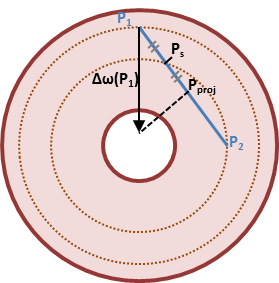
\includegraphics[width=0.35\textwidth]{Drawings/ProjectionTest.png}
%%\caption{The gradient of potential at $P_1$ is projected along the segment $p_1p_2$. The sampling distance is calculated as half way.}
%%\label{projectiontest}
%%\end{figure}





\bibliography{notes_ht.bib}
\bibliographystyle{plain}
	
\end{document}